\pdfinfoomitdate=1
\pdftrailerid{}
\pdfsuppressptexinfo=-1
\documentclass[11pt]{article}
\usepackage[margin=0.78in]{geometry}
\usepackage{booktabs}
\usepackage{graphicx}
\usepackage{hyperref}
\usepackage{xcolor}
\usepackage{amsmath}
\hypersetup{colorlinks=true,linkcolor=blue,urlcolor=blue}
\setlength{\parindent}{0pt}
\setlength{\parskip}{0.55em}
\setlength{\emergencystretch}{3em}

\newcommand{\code}[1]{\texttt{\detokenize{#1}}}

\title{AthenaK Figure-3 Brill Evolution:\\
Telegrapher and Gamma-driver Damping Diagnostics}
\author{Authenticated numerical investigation bundle}
\date{14 August 2026}

\begin{document}
\maketitle

\begin{abstract}
This report consolidates five matched AthenaK evolutions of the $A=-0.047$
Brill initial data used in the Figure-3 reproduction study.  Four runs compare
prospectively selected scale-invariant telegrapher damping fields.  A fifth,
single controlled diagnostic changes only the Gamma-driver shift damping from
$\eta=2\max|K|$ to fixed $\eta=2$.  The fixed-$\eta$ control strongly implicates
the global $\max|K|$ shift scaling in the baseline's late stiffness, but the
control itself develops a different central curvature/constraint pathology and
is neither a robust solution nor scale invariant.  No coefficient sweep,
threshold relaxation, floor, clipping, or selective rerun was used.
\end{abstract}

\section{Common Figure-3 configuration}

All cases use the same IrisK global $48\times32$ coefficient payload, directly
interpolated by AthenaK without an M0 intermediate-domain reconstruction.  The
Brill amplitude is $A=-0.047$ and the imported ADM mass is
$2.660301967997158$.  The initial lapse is pre-collapsed,
$\alpha=\psi^{-2}$.  Evolution uses the $\rho\geq0$ Cartoon half-plane,
$N128$, sixth-order spatial operators, RK4, CFL $0.15$, KO dissipation $0.02$,
nine available AMR levels, and $d\chi_{\max}=0.02$.  The strict-positive chi
gate is unchanged and \code{floor_chi=false}.  The lapse is the telegrapher
gauge with $\tau=\kappa=1$ and the domain-$\max|K|$ prescription unless stated
otherwise.  Z4c damping remains enabled with its existing max-$K$ scaling.

The source for all five runs is:
\begin{quote}\small
commit: \code{2a8ad80e02279769a99fe279b7a33516bc6c8d0d}\\
tree: \code{67709c405a1169a15643cb933eec5353cd216243}\\
Kokkos: \code{6739bc623081648af9e752b616d9671527922cbf}
\end{quote}

\section{Local telegrapher-scale comparison}

The four prospectively fixed inverse-length fields were
\[
 \mu\in\left\{\max_\Omega|K|,\ |K(x)|,\
 \sqrt{K_{ij}K^{ij}},\
 \sqrt{\gamma^{ij}\partial_i\chi\partial_j\chi}\right\}.
\]
With $K_\star=\max_\Omega|K|$, the conceptual scaling is
\[
 Q=\frac{\mu}{K_\star},\qquad
 \tau_{\rm eff}=\frac{\tau}{K_\star},\qquad
 \kappa_{\rm eff}=\frac{\kappa}{K_\star}.
\]
The kernel evaluates the cancelled ratios $Q/\tau_{\rm eff}=\mu/\tau$ and
$\kappa_{\rm eff}/\tau_{\rm eff}=\kappa/\tau$, providing a finite extension
through the time-symmetric initial slice.

\begin{center}
\begin{tabular}{lrrr}
\toprule
telegrapher damping field & terminal $t/M$ & terminal $\tau/M$ & rejected parents\\
\midrule
$\max_\Omega|K|$ & 10.162940 & 6.201069 & 6412\\
$|K(x)|$ & 8.907275 & 5.472376 & 13184\\
$\sqrt{K_{ij}K^{ij}}$ & 9.193945 & 5.751011 & 12\\
$|\nabla\chi|_\gamma$ & 8.358252 & 5.016554 & 7320\\
\bottomrule
\end{tabular}
\end{center}

All four runs stopped at the unchanged positive-chi boundary-prolongation
gate.  The rejected-parent count is an inventory at different physical states,
not a stability ranking.  The domain-maximum case remains the best comparator
among these four; none is a qualified Figure-3 evolution.

\begin{figure}[p]
\centering
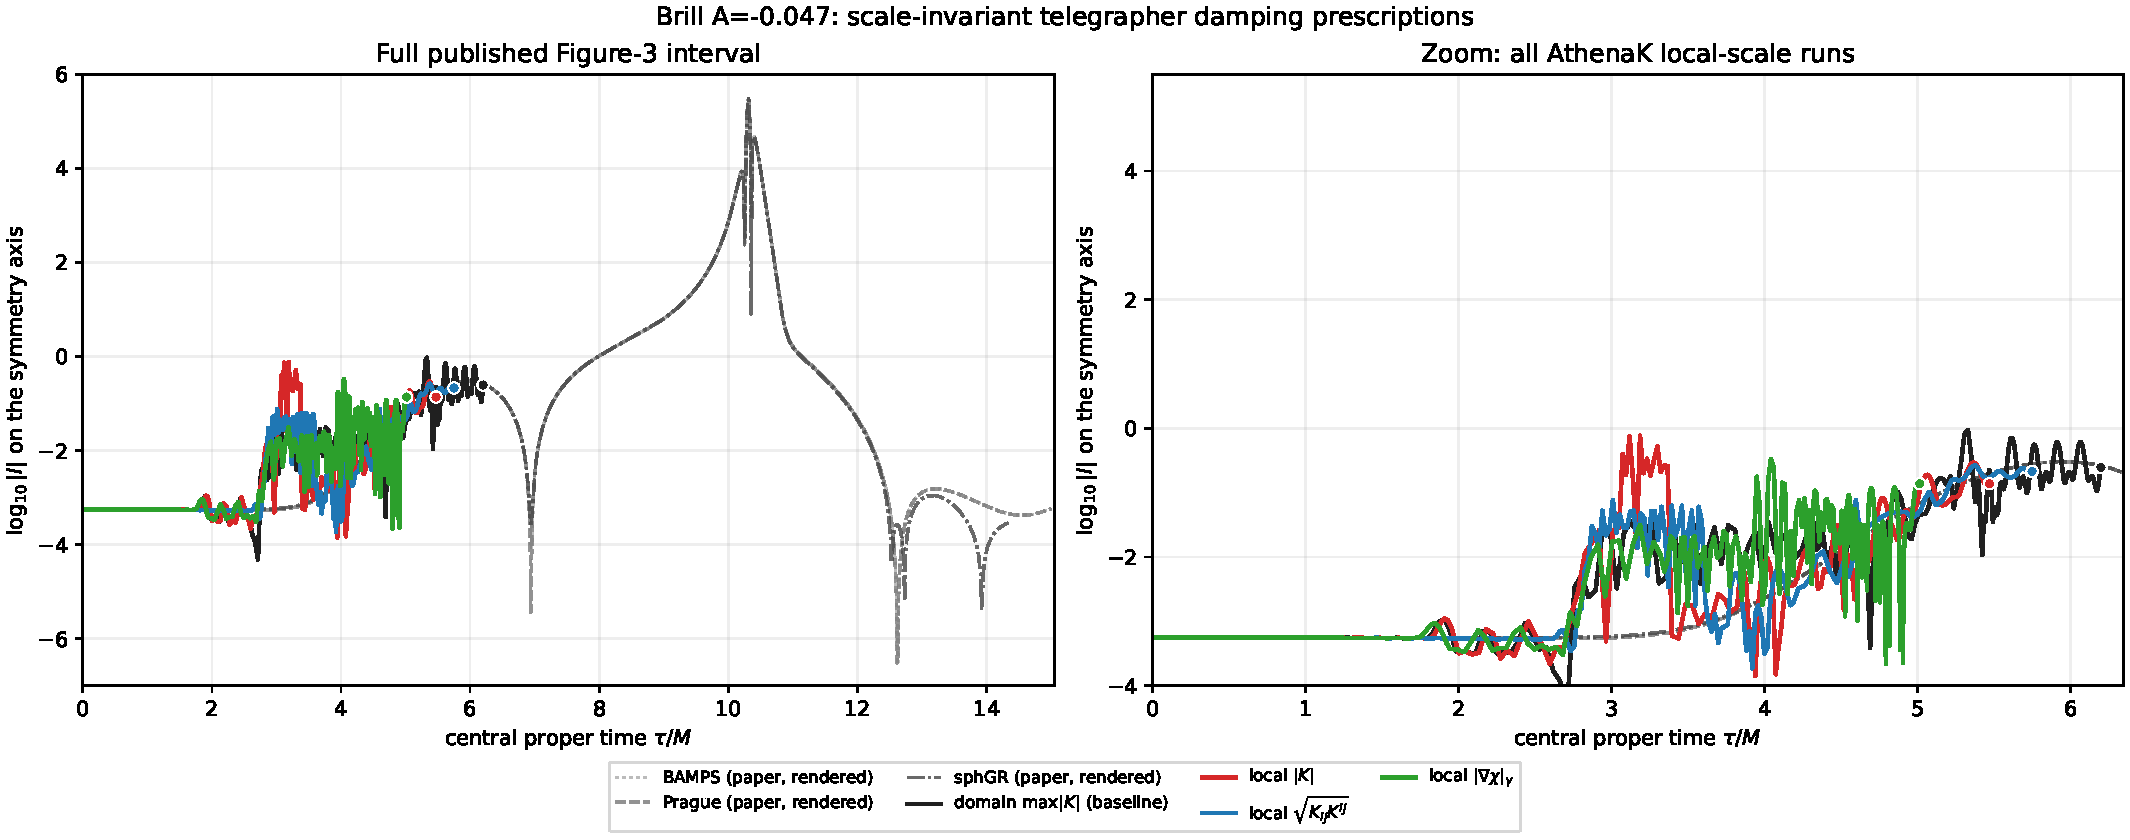
\includegraphics[width=0.98\textwidth]{figures/figure3_local_telegraph_mu_comparison.pdf}
\caption{The four scale-invariant telegrapher damping choices plotted on the
rendered Figure-3 axes.  All terminate before covering the published interval.}
\end{figure}

\section{Fixed-shift control}

The controlled follow-up changes exactly one runtime setting:
\[
 \code{z4c/shift_eta_max_K=true}\quad\longrightarrow\quad
 \code{z4c/shift_eta_max_K=false}.
\]
Thus the baseline has $\eta_{\rm shift}=2\max|K|$ while the control has fixed
$\eta_{\rm shift}=2$.  The source, executable, input, initial-data payload,
telegrapher lapse, Z4c damping, mesh, AMR, timestep controls, and numerical
thresholds are identical.

Define the explicit RK damping stiffness number
\[
 S_\beta=\Delta t\,\eta_{\rm shift}.
\]
The baseline reaches $S_\beta=5.55889$, exceeding the approximate RK4
negative-real-axis limit $2.8$, immediately before its chi-gate failure.  The
fixed-$\eta$ control never exceeds $S_\beta=0.075$.

At the baseline terminal time, the fixed-$\eta$ evolution remains controlled:
its combined constraint norm is $136.6$ rather than $2.40\times10^{11}$,
$\max|K|=3.49$ rather than $1.90\times10^4$, sampled
$\max|\widetilde\Gamma|=0.237$ rather than $1288$, and it uses 32 rather than
290 MeshBlocks.  Central lapse and central proper time remain closely matched.

The fixed-$\eta$ case avoids the chi rejection and reaches $t=16.73892M$,
$\tau=10.37631M$: $6.57598M$ or $64.7\%$ farther in coordinate time.  It then
fails a different strict diagnostic after cycle 2333 because axis-central
physical support becomes nonfinite or invalid.  The last finite row already
has $\max|K|=1.0689\times10^4$, axis Kretschmann
$7.6154\times10^{15}$, and combined constraint norm
$8.3439\times10^7$.  The frozen telemetry does not identify whether lapse,
constraint density, or curvature reconstruction becomes invalid first.

\begin{figure}[p]
\centering
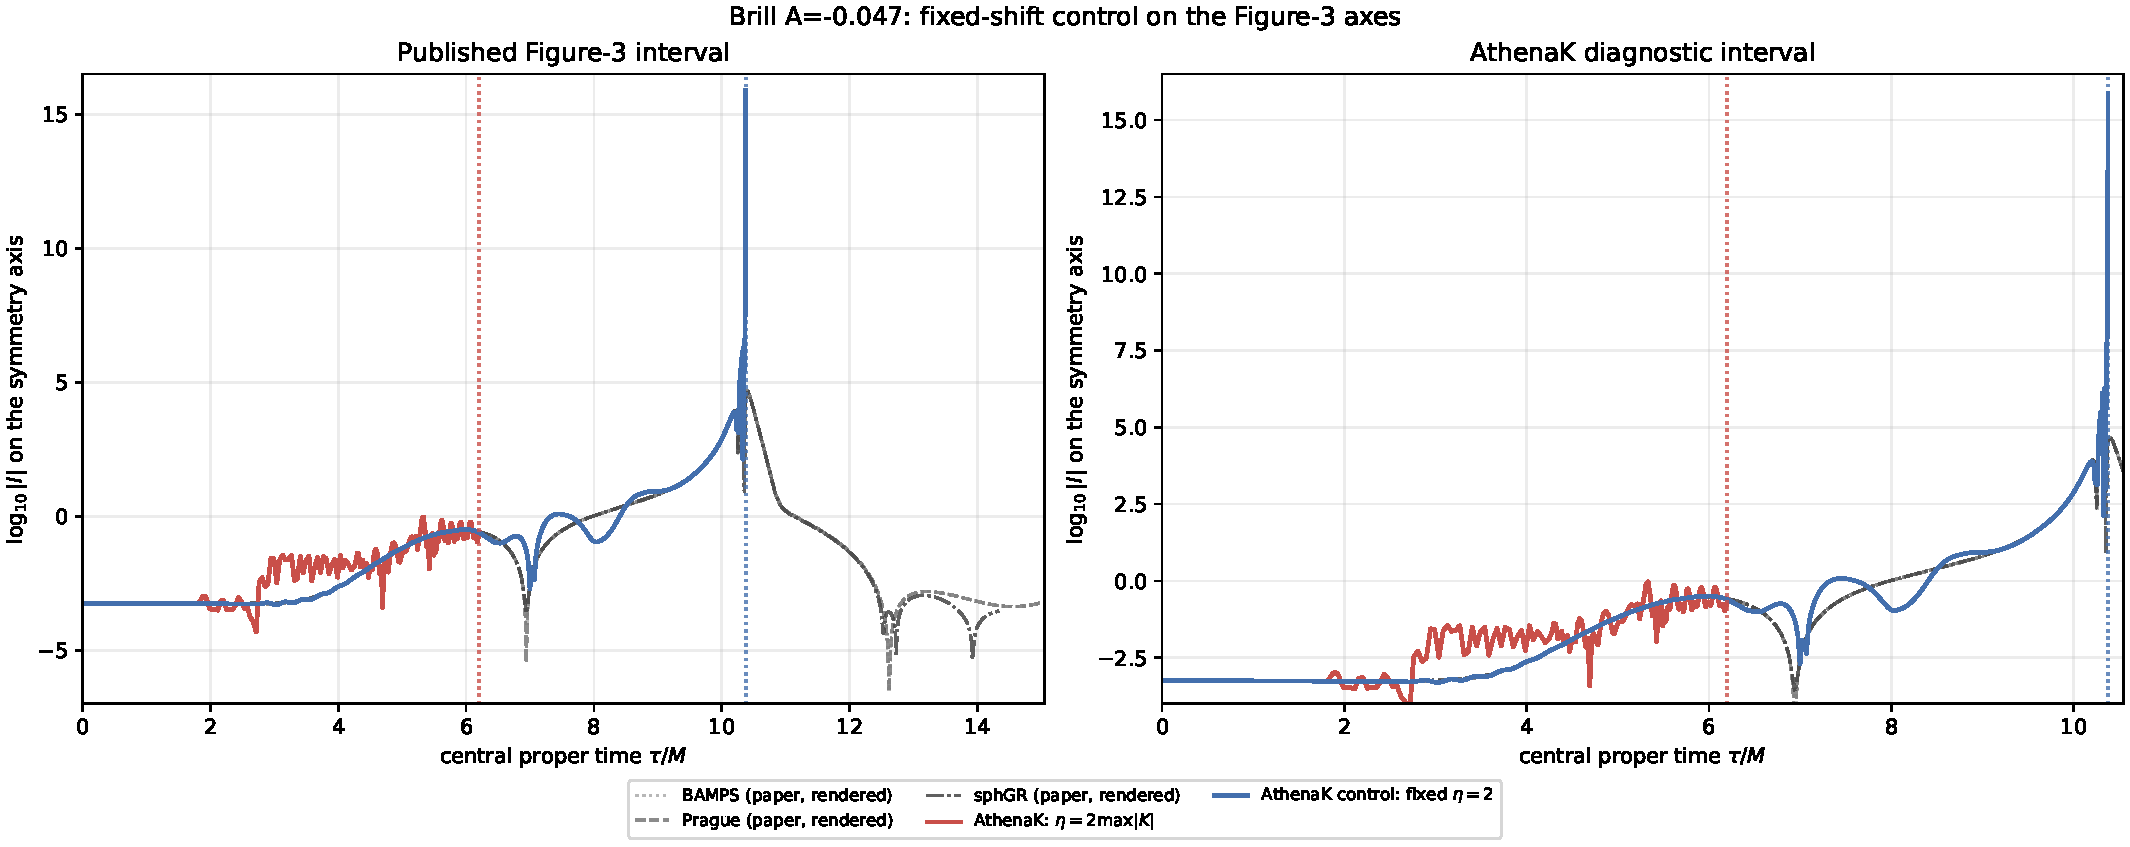
\includegraphics[width=0.98\textwidth]{figures/figure3_fixed_shift_eta2_overlay.pdf}
\caption{The fixed-$\eta$ control added directly to the Figure-3 reproduction
axes.  The dotted vertical lines show the last finite baseline and control
history rows.  Longer survival is diagnostic evidence, not reproduction or
convergence.}
\end{figure}

\begin{figure}[p]
\centering
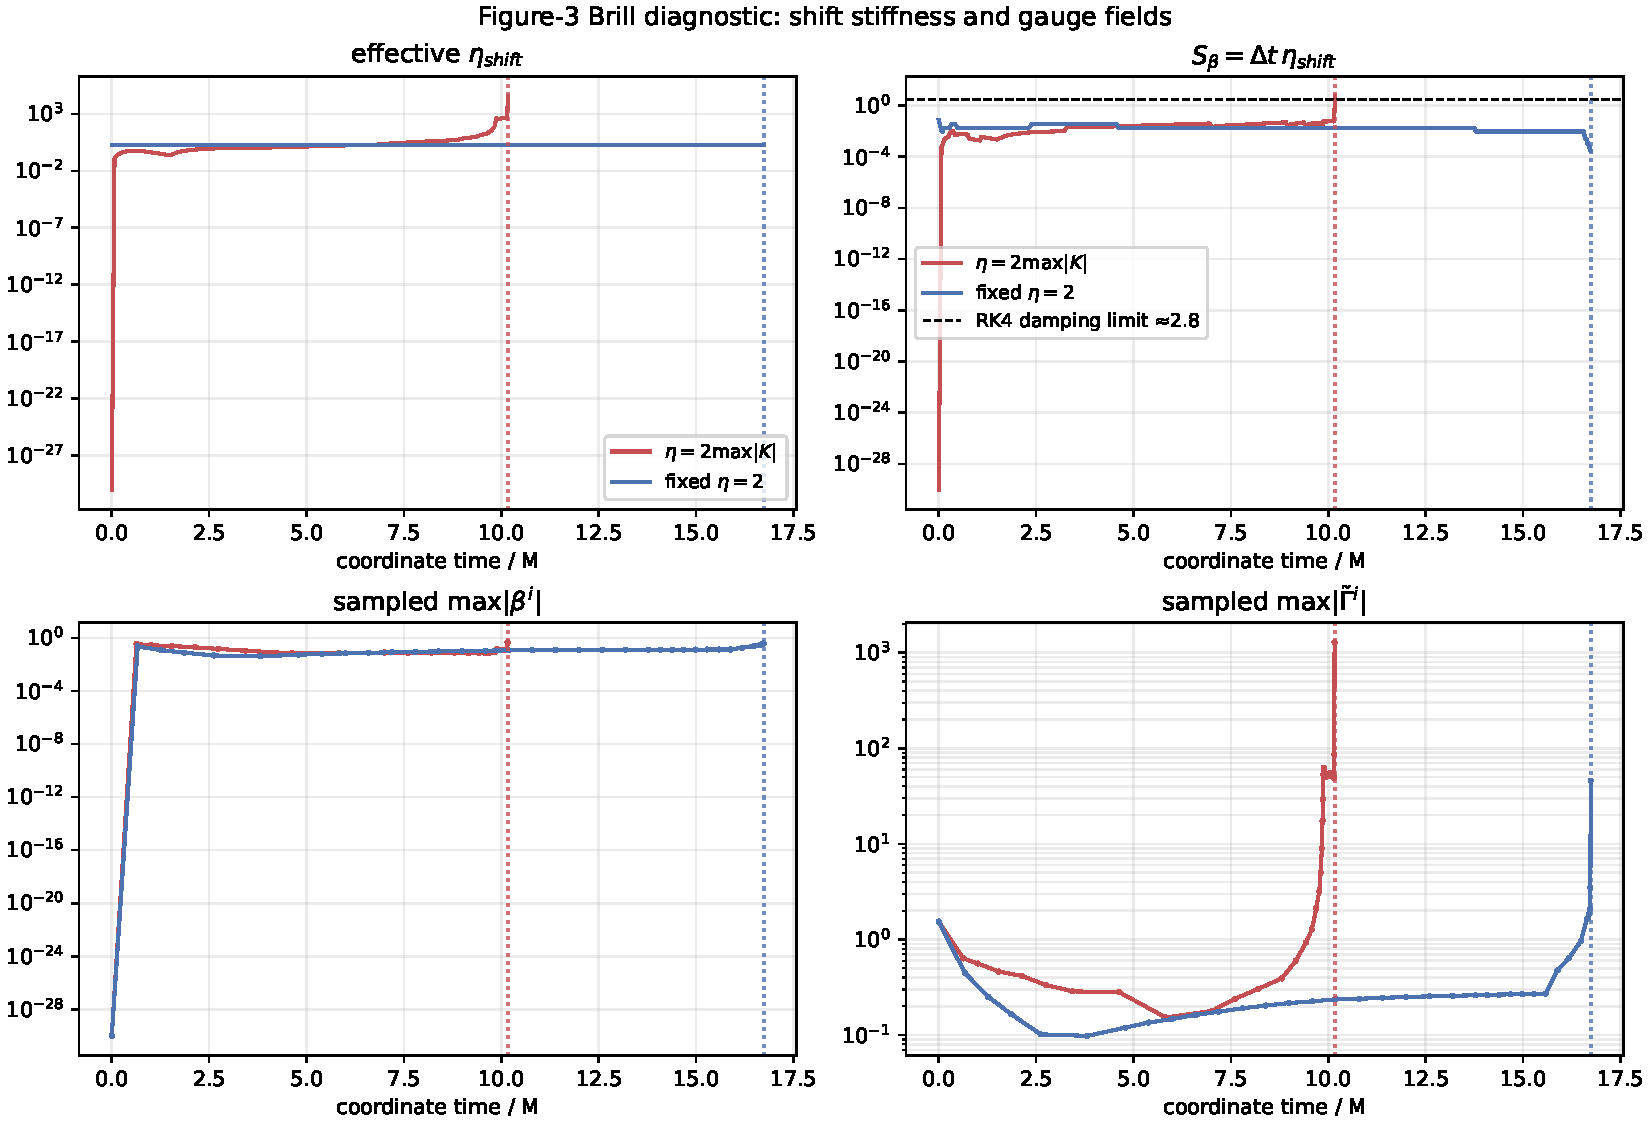
\includegraphics[width=0.98\textwidth]{figures/fixed_shift_eta2_stiffness_and_gauge.pdf}
\caption{Effective shift damping, stiffness number, and sampled shift and
conformal-connection extrema.  The fixed control removes the baseline RK4
damping-axis violation but later develops its own growth.}
\end{figure}

\begin{figure}[p]
\centering
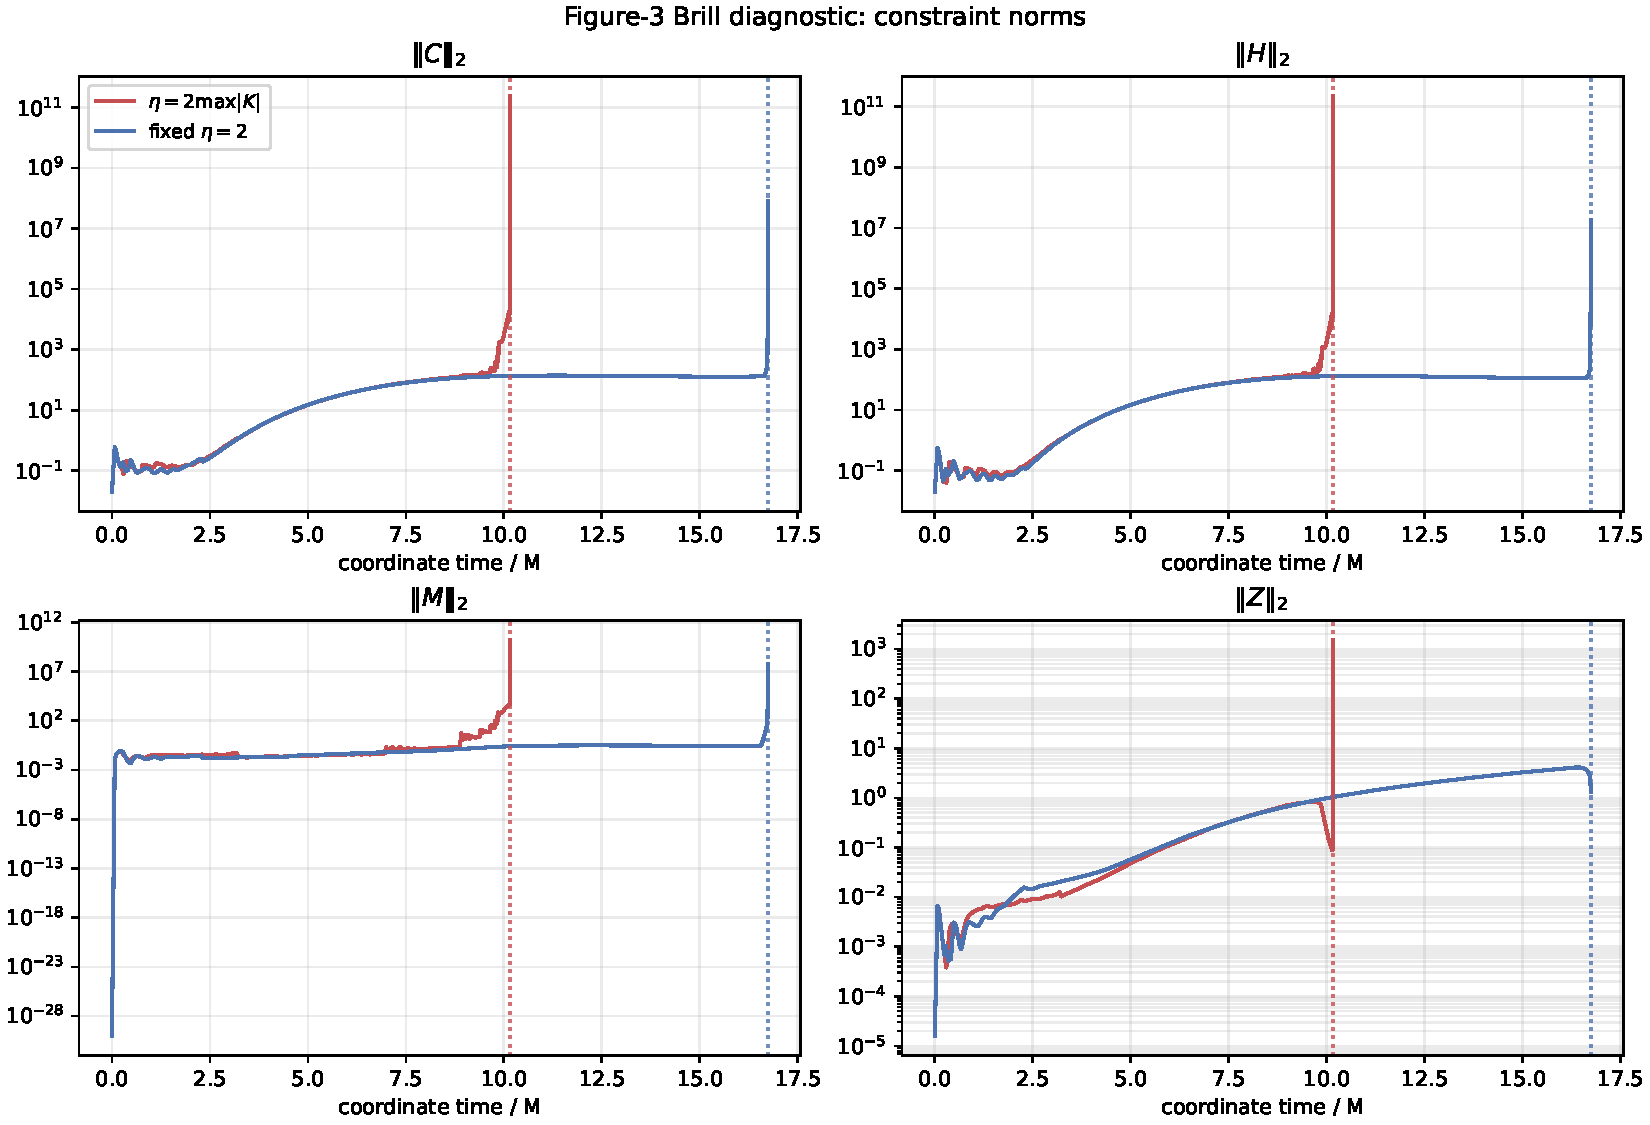
\includegraphics[width=0.98\textwidth]{figures/fixed_shift_eta2_constraint_comparison.pdf}
\caption{Constraint histories for the matched baseline and fixed-$\eta$
control.  The control stays orders of magnitude smaller at the baseline
failure time, then grows rapidly near its distinct terminal event.}
\end{figure}

\begin{figure}[p]
\centering
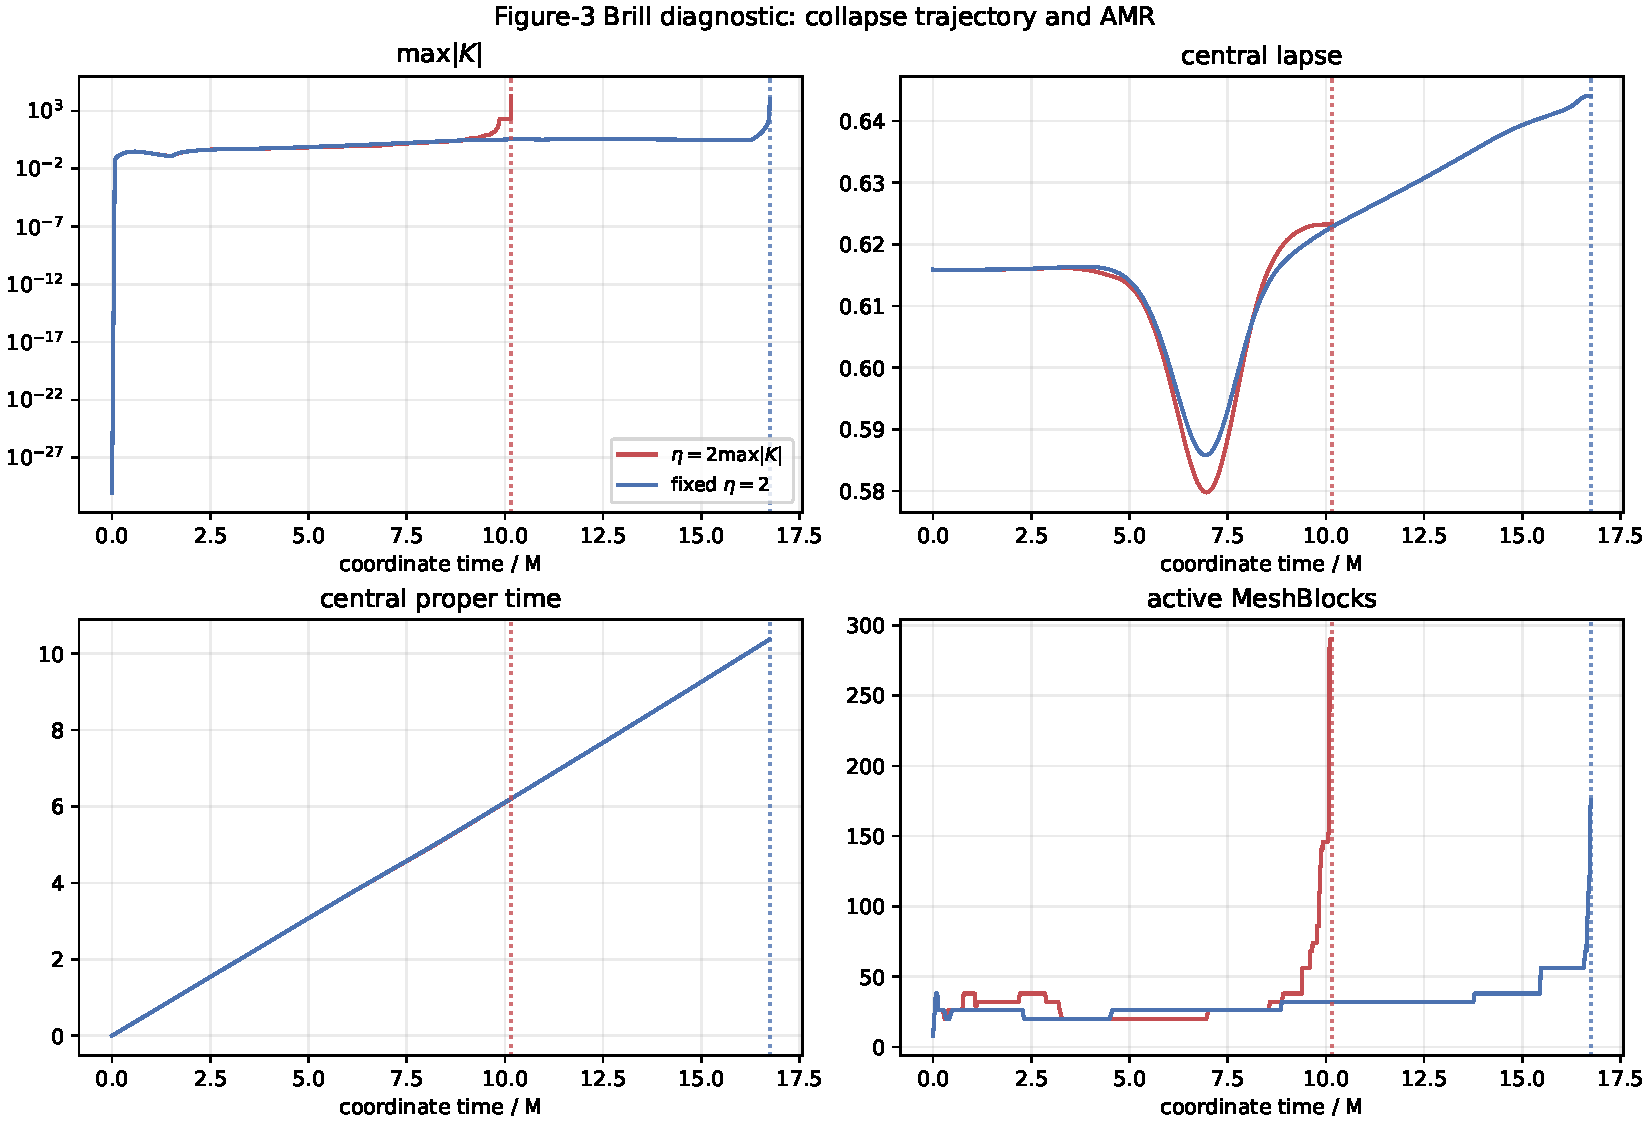
\includegraphics[width=0.98\textwidth]{figures/fixed_shift_eta2_trajectory_and_amr.pdf}
\caption{Collapse trajectory and AMR inventory.  The two evolutions track
closely at early times, separate before the baseline failure, and both end in
unqualified late-time pathologies.}
\end{figure}

\section{Interpretation and qualification boundary}

The controlled result is strong evidence that global $\max|K|$-scaled
Gamma-driver damping is a major contributor to the baseline stiffness and
$t\simeq10.16M$ failure.  The causal case is not based merely on later
survival: the sole parameter change prevents the RK4 damping violation and
suppresses the accompanying $\widetilde\Gamma$, constraint, and AMR explosion
at matched time.

It does not establish that shift scaling is the only failure mechanism.  Fixed
$\eta=2$ introduces a dimensionful scale, violates the target scale-invariance
principle, and ends in a central curvature/constraint pathology.  Consequently
the result supports redesigning the shift damping scale; it does not support
adopting fixed $\eta$, weakening the chi gate, or claiming Figure-3
reproduction.  The report makes no convergence, horizon, or production
qualification claim.

The smallest useful next reasoning task is mathematical rather than another
parameter sweep: construct a smooth positive inverse-length functional for
the shift whose induced $\Delta t\,\eta$ remains bounded while preserving mass
rescaling, and identify a prospective diagnostic that distinguishes gauge
stiffness from the later central curvature failure.

\section{Provenance}

The four-mode campaign is Perlmutter job \code{56955603}.  The fixed-$\eta$
control is job \code{56966125}.  Its key SHA-256 identities are:
\begin{quote}\small
executable: \code{8325bd78f4851f04e6810aaf9fb5ecfc4007d876c3a3011a296512ffbd7875be}\\
root manifest: \code{29acd8986ce53afbb8bf472b70e09f554e224c640977528a421ffb0558713fba}\\
detached manifest: \code{ce2136a1a81f1cd06cab592240147359732805aea72b837f8417c6ad7fb8c07d}
\end{quote}
The fixed-control result JSON and reduced CSVs in this directory are sufficient
to reproduce every plot in this report without native AthenaK binaries.

\end{document}
